\documentclass{standalone}
\usepackage{tikz}
\usetikzlibrary{patterns}
\usetikzlibrary{positioning}
\usetikzlibrary{patterns, positioning}
\usetikzlibrary{shapes.misc}
\usepackage[outline]{contour}
\contourlength{1.5pt} 


\begin{document}
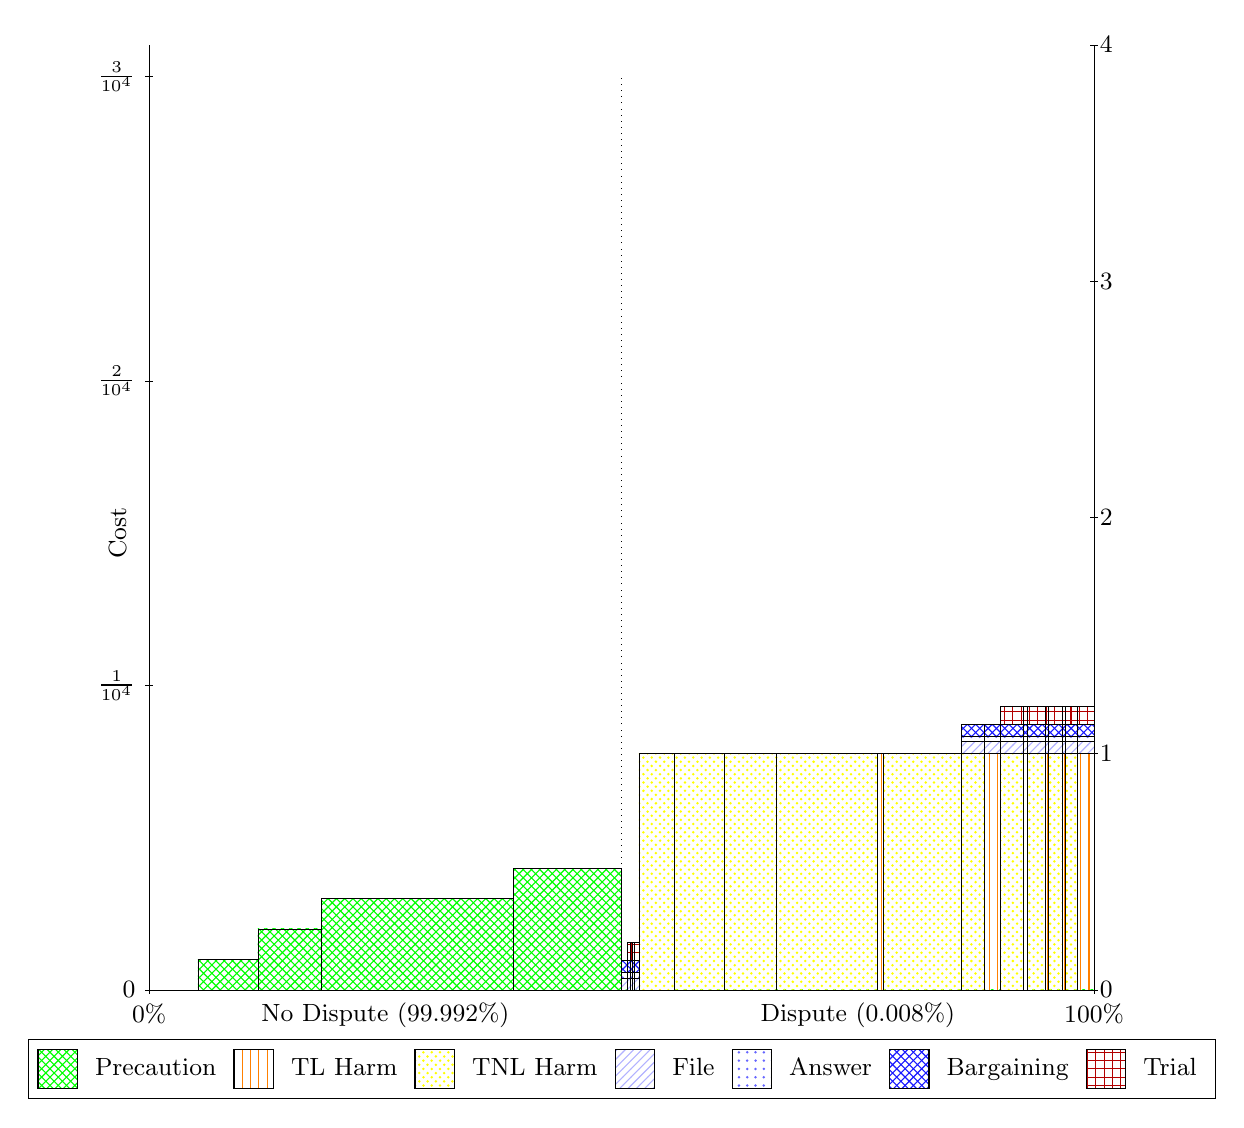
\begin{tikzpicture}
\draw[pattern=crosshatch, pattern color=green,draw=black,very thin] (2.117,2.5) rectangle (2.8801,2.8866);
\draw[pattern=crosshatch, pattern color=green,draw=black,very thin] (2.8801,2.5) rectangle (3.6907,3.2733);
\draw[pattern=crosshatch, pattern color=green,draw=black,very thin] (3.6907,2.5) rectangle (6.1199,3.6599);
\draw[pattern=crosshatch, pattern color=green,draw=black,very thin] (6.1199,2.5) rectangle (7.5,4.0466);
\draw[pattern=crosshatch, pattern color=green,draw=black,very thin] (7.5,2.5) rectangle (7.5736,2.5001);
\draw[pattern=north east lines, pattern color=blue!30,draw=black,very thin] (7.5,2.5001) rectangle (7.5736,2.6501);
\draw[pattern=dots,  pattern color=blue!60,draw=black,very thin] (7.5,2.6501) rectangle (7.5736,2.7251);
\draw[pattern=crosshatch,      pattern color=blue!90,draw=black,very thin] (7.5,2.7251) rectangle (7.5736,2.8751);
\draw[pattern=north east lines, pattern color=blue!30,draw=black,very thin] (7.5736,2.5) rectangle (7.6079,2.65);
\draw[pattern=dots,  pattern color=blue!60,draw=black,very thin] (7.5736,2.65) rectangle (7.6079,2.725);
\draw[pattern=crosshatch,      pattern color=blue!90,draw=black,very thin] (7.5736,2.725) rectangle (7.6079,2.875);
\draw[pattern=grid,            pattern color=red!70!black,draw=black,very thin] (7.5736,2.875) rectangle (7.6079,3.1);
\draw[pattern=crosshatch, pattern color=green,draw=black,very thin] (7.6079,2.5) rectangle (7.6376,2.5);
\draw[pattern=north east lines, pattern color=blue!30,draw=black,very thin] (7.6079,2.5) rectangle (7.6376,2.65);
\draw[pattern=dots,  pattern color=blue!60,draw=black,very thin] (7.6079,2.65) rectangle (7.6376,2.725);
\draw[pattern=crosshatch,      pattern color=blue!90,draw=black,very thin] (7.6079,2.725) rectangle (7.6376,2.875);
\draw[pattern=grid,            pattern color=red!70!black,draw=black,very thin] (7.6079,2.875) rectangle (7.6376,3.1);
\draw[pattern=crosshatch, pattern color=green,draw=black,very thin] (7.6376,2.5) rectangle (7.6643,2.5001);
\draw[pattern=north east lines, pattern color=blue!30,draw=black,very thin] (7.6376,2.5001) rectangle (7.6643,2.6501);
\draw[pattern=dots,  pattern color=blue!60,draw=black,very thin] (7.6376,2.6501) rectangle (7.6643,2.7251);
\draw[pattern=crosshatch,      pattern color=blue!90,draw=black,very thin] (7.6376,2.7251) rectangle (7.6643,2.8751);
\draw[pattern=grid,            pattern color=red!70!black,draw=black,very thin] (7.6376,2.8751) rectangle (7.6643,3.1001);
\draw[pattern=crosshatch, pattern color=green,draw=black,very thin] (7.6643,2.5) rectangle (7.7192,2.5001);
\draw[pattern=north east lines, pattern color=blue!30,draw=black,very thin] (7.6643,2.5001) rectangle (7.7192,2.6501);
\draw[pattern=dots,  pattern color=blue!60,draw=black,very thin] (7.6643,2.6501) rectangle (7.7192,2.7251);
\draw[pattern=crosshatch,      pattern color=blue!90,draw=black,very thin] (7.6643,2.7251) rectangle (7.7192,2.8751);
\draw[pattern=grid,            pattern color=red!70!black,draw=black,very thin] (7.6643,2.8751) rectangle (7.7192,3.1001);
\draw[pattern=crosshatch dots, pattern color=yellow,draw=black,very thin] (7.7192,2.5) rectangle (8.1646,5.5);
\draw[pattern=vertical lines, pattern color=orange,draw=black,very thin] (8.1646,2.5) rectangle (8.1705,5.5);
\draw[pattern=crosshatch, pattern color=green,draw=black,very thin] (8.1705,2.5) rectangle (8.8019,2.5);
\draw[pattern=crosshatch dots, pattern color=yellow,draw=black,very thin] (8.1705,2.5) rectangle (8.8019,5.5);
\draw[pattern=crosshatch, pattern color=green,draw=black,very thin] (8.8019,2.5) rectangle (8.8076,2.5);
\draw[pattern=vertical lines, pattern color=orange,draw=black,very thin] (8.8019,2.5) rectangle (8.8076,5.5);
\draw[pattern=crosshatch, pattern color=green,draw=black,very thin] (8.8076,2.5) rectangle (9.4597,2.5001);
\draw[pattern=crosshatch dots, pattern color=yellow,draw=black,very thin] (8.8076,2.5001) rectangle (9.4597,5.5001);
\draw[pattern=crosshatch, pattern color=green,draw=black,very thin] (9.4597,2.5) rectangle (9.4661,2.5001);
\draw[pattern=vertical lines, pattern color=orange,draw=black,very thin] (9.4597,2.5001) rectangle (9.4661,5.5001);
\draw[pattern=crosshatch, pattern color=green,draw=black,very thin] (9.4661,2.5) rectangle (10.74,2.5001);
\draw[pattern=crosshatch dots, pattern color=yellow,draw=black,very thin] (9.4661,2.5001) rectangle (10.74,5.5001);
\draw[pattern=crosshatch, pattern color=green,draw=black,very thin] (10.74,2.5) rectangle (10.821,2.5001);
\draw[pattern=vertical lines, pattern color=orange,draw=black,very thin] (10.74,2.5001) rectangle (10.821,5.5001);
\draw[pattern=crosshatch, pattern color=green,draw=black,very thin] (10.821,2.5) rectangle (11.812,2.5001);
\draw[pattern=crosshatch dots, pattern color=yellow,draw=black,very thin] (10.821,2.5001) rectangle (11.812,5.5001);
\draw[pattern=crosshatch, pattern color=green,draw=black,very thin] (11.812,2.5) rectangle (12.103,2.5001);
\draw[pattern=crosshatch dots, pattern color=yellow,draw=black,very thin] (11.812,2.5001) rectangle (12.103,5.5001);
\draw[pattern=north east lines, pattern color=blue!30,draw=black,very thin] (11.812,5.5001) rectangle (12.103,5.6501);
\draw[pattern=dots,  pattern color=blue!60,draw=black,very thin] (11.812,5.6501) rectangle (12.103,5.7251);
\draw[pattern=crosshatch,      pattern color=blue!90,draw=black,very thin] (11.812,5.7251) rectangle (12.103,5.8751);
\draw[pattern=crosshatch, pattern color=green,draw=black,very thin] (12.103,2.5) rectangle (12.308,2.5001);
\draw[pattern=vertical lines, pattern color=orange,draw=black,very thin] (12.103,2.5001) rectangle (12.308,5.5001);
\draw[pattern=north east lines, pattern color=blue!30,draw=black,very thin] (12.103,5.5001) rectangle (12.308,5.6501);
\draw[pattern=dots,  pattern color=blue!60,draw=black,very thin] (12.103,5.6501) rectangle (12.308,5.7251);
\draw[pattern=crosshatch,      pattern color=blue!90,draw=black,very thin] (12.103,5.7251) rectangle (12.308,5.8751);
\draw[pattern=crosshatch dots, pattern color=yellow,draw=black,very thin] (12.308,2.5) rectangle (12.606,5.5);
\draw[pattern=north east lines, pattern color=blue!30,draw=black,very thin] (12.308,5.5) rectangle (12.606,5.65);
\draw[pattern=dots,  pattern color=blue!60,draw=black,very thin] (12.308,5.65) rectangle (12.606,5.725);
\draw[pattern=crosshatch,      pattern color=blue!90,draw=black,very thin] (12.308,5.725) rectangle (12.606,5.875);
\draw[pattern=grid,            pattern color=red!70!black,draw=black,very thin] (12.308,5.875) rectangle (12.606,6.1);
\draw[pattern=vertical lines, pattern color=orange,draw=black,very thin] (12.606,2.5) rectangle (12.652,5.5);
\draw[pattern=north east lines, pattern color=blue!30,draw=black,very thin] (12.606,5.5) rectangle (12.652,5.65);
\draw[pattern=dots,  pattern color=blue!60,draw=black,very thin] (12.606,5.65) rectangle (12.652,5.725);
\draw[pattern=crosshatch,      pattern color=blue!90,draw=black,very thin] (12.606,5.725) rectangle (12.652,5.875);
\draw[pattern=grid,            pattern color=red!70!black,draw=black,very thin] (12.606,5.875) rectangle (12.652,6.1);
\draw[pattern=crosshatch, pattern color=green,draw=black,very thin] (12.652,2.5) rectangle (12.878,2.5);
\draw[pattern=crosshatch dots, pattern color=yellow,draw=black,very thin] (12.652,2.5) rectangle (12.878,5.5);
\draw[pattern=north east lines, pattern color=blue!30,draw=black,very thin] (12.652,5.5) rectangle (12.878,5.65);
\draw[pattern=dots,  pattern color=blue!60,draw=black,very thin] (12.652,5.65) rectangle (12.878,5.725);
\draw[pattern=crosshatch,      pattern color=blue!90,draw=black,very thin] (12.652,5.725) rectangle (12.878,5.875);
\draw[pattern=grid,            pattern color=red!70!black,draw=black,very thin] (12.652,5.875) rectangle (12.878,6.1);
\draw[pattern=crosshatch, pattern color=green,draw=black,very thin] (12.878,2.5) rectangle (12.922,2.5);
\draw[pattern=vertical lines, pattern color=orange,draw=black,very thin] (12.878,2.5) rectangle (12.922,5.5);
\draw[pattern=north east lines, pattern color=blue!30,draw=black,very thin] (12.878,5.5) rectangle (12.922,5.65);
\draw[pattern=dots,  pattern color=blue!60,draw=black,very thin] (12.878,5.65) rectangle (12.922,5.725);
\draw[pattern=crosshatch,      pattern color=blue!90,draw=black,very thin] (12.878,5.725) rectangle (12.922,5.875);
\draw[pattern=grid,            pattern color=red!70!black,draw=black,very thin] (12.878,5.875) rectangle (12.922,6.1);
\draw[pattern=crosshatch, pattern color=green,draw=black,very thin] (12.922,2.5) rectangle (13.095,2.5001);
\draw[pattern=crosshatch dots, pattern color=yellow,draw=black,very thin] (12.922,2.5001) rectangle (13.095,5.5001);
\draw[pattern=north east lines, pattern color=blue!30,draw=black,very thin] (12.922,5.5001) rectangle (13.095,5.6501);
\draw[pattern=dots,  pattern color=blue!60,draw=black,very thin] (12.922,5.6501) rectangle (13.095,5.7251);
\draw[pattern=crosshatch,      pattern color=blue!90,draw=black,very thin] (12.922,5.7251) rectangle (13.095,5.8751);
\draw[pattern=grid,            pattern color=red!70!black,draw=black,very thin] (12.922,5.8751) rectangle (13.095,6.1001);
\draw[pattern=crosshatch, pattern color=green,draw=black,very thin] (13.095,2.5) rectangle (13.137,2.5001);
\draw[pattern=vertical lines, pattern color=orange,draw=black,very thin] (13.095,2.5001) rectangle (13.137,5.5001);
\draw[pattern=north east lines, pattern color=blue!30,draw=black,very thin] (13.095,5.5001) rectangle (13.137,5.6501);
\draw[pattern=dots,  pattern color=blue!60,draw=black,very thin] (13.095,5.6501) rectangle (13.137,5.7251);
\draw[pattern=crosshatch,      pattern color=blue!90,draw=black,very thin] (13.095,5.7251) rectangle (13.137,5.8751);
\draw[pattern=grid,            pattern color=red!70!black,draw=black,very thin] (13.095,5.8751) rectangle (13.137,6.1001);
\draw[pattern=crosshatch, pattern color=green,draw=black,very thin] (13.137,2.5) rectangle (13.292,2.5001);
\draw[pattern=crosshatch dots, pattern color=yellow,draw=black,very thin] (13.137,2.5001) rectangle (13.292,5.5001);
\draw[pattern=north east lines, pattern color=blue!30,draw=black,very thin] (13.137,5.5001) rectangle (13.292,5.6501);
\draw[pattern=dots,  pattern color=blue!60,draw=black,very thin] (13.137,5.6501) rectangle (13.292,5.7251);
\draw[pattern=crosshatch,      pattern color=blue!90,draw=black,very thin] (13.137,5.7251) rectangle (13.292,5.8751);
\draw[pattern=grid,            pattern color=red!70!black,draw=black,very thin] (13.137,5.8751) rectangle (13.292,6.1001);
\draw[pattern=crosshatch, pattern color=green,draw=black,very thin] (13.292,2.5) rectangle (13.5,2.5001);
\draw[pattern=vertical lines, pattern color=orange,draw=black,very thin] (13.292,2.5001) rectangle (13.5,5.5001);
\draw[pattern=north east lines, pattern color=blue!30,draw=black,very thin] (13.292,5.5001) rectangle (13.5,5.6501);
\draw[pattern=dots,  pattern color=blue!60,draw=black,very thin] (13.292,5.6501) rectangle (13.5,5.7251);
\draw[pattern=crosshatch,      pattern color=blue!90,draw=black,very thin] (13.292,5.7251) rectangle (13.5,5.8751);
\draw[pattern=grid,            pattern color=red!70!black,draw=black,very thin] (13.292,5.8751) rectangle (13.5,6.1001);
\draw[black,very thin] (1.5,2.5) -- (1.5,14.5);
\node[font=\small,rotate=90,text=black, anchor=center] at (1.1, 8.2996) {Cost};
\draw[black,very thin] (1.45,2.5) -- (1.55,2.5);
\node[font=\small,text=black, anchor=east] at (1.45, 2.5) {0};
\draw[black,very thin] (1.45,6.3664) -- (1.55,6.3664);
\node[font=\small,text=black, anchor=east] at (1.45, 6.3664) {$\frac{1}{10^{4}}$};
\draw[black,very thin] (1.45,10.233) -- (1.55,10.233);
\node[font=\small,text=black, anchor=east] at (1.45, 10.233) {$\frac{2}{10^{4}}$};
\draw[black,very thin] (1.45,14.099) -- (1.55,14.099);
\node[font=\small,text=black, anchor=east] at (1.45, 14.099) {$\frac{3}{10^{4}}$};

\draw[black,dotted,very thin] (7.5,2.86) -- (7.5,14.14);
\draw[black,very thin] (13.5,2.5) -- (13.5,14.5);
\draw[black,very thin] (13.45,2.5) -- (13.55,2.5);
\node[font=\small,text=black, anchor=west] at (13.45, 2.5) {0};
\draw[black,very thin] (13.45,5.5) -- (13.55,5.5);
\node[font=\small,text=black, anchor=west] at (13.45, 5.5) {1};
\draw[black,very thin] (13.45,8.5) -- (13.55,8.5);
\node[font=\small,text=black, anchor=west] at (13.45, 8.5) {2};
\draw[black,very thin] (13.45,11.5) -- (13.55,11.5);
\node[font=\small,text=black, anchor=west] at (13.45, 11.5) {3};
\draw[black,very thin] (13.45,14.5) -- (13.55,14.5);
\node[font=\small,text=black, anchor=west] at (13.45, 14.5) {4};

\draw[black,very thin] (1.5,2.5) -- (13.5,2.5);
\draw[black,very thin] (1.5,2.45) -- (1.5,2.55);
\node[font=\small,text=black, anchor=north] at (1.5, 2.45) {0\%};
\draw[black,very thin] (13.5,2.45) -- (13.5,2.55);
\node[font=\small,text=black, anchor=north] at (13.5, 2.45) {100\%};

\node[font=\small,text=black,anchor=south] at (4.5, 1.9) {No\ Dispute\ (99.992\%)};
\node[font=\small,text=black,anchor=south] at (10.5, 1.9) {Dispute\ (0.008\%)};
\draw (7.5,2.5) node (B) {};
\begin{scope}[align=center]
\matrix[scale=0.5,draw=black,below=0.5cm of B,nodes={draw},column sep=0.1cm]{
\node[rectangle,draw,minimum width=0.5cm,minimum height=0.5cm,pattern=crosshatch, pattern color=green]{}; & \node[draw=none,font=\small,text=black]{Precaution}; &
\node[rectangle,draw,minimum width=0.5cm,minimum height=0.5cm,pattern=vertical lines, pattern color=orange]{}; & \node[draw=none,font=\small,text=black]{TL Harm}; &
\node[rectangle,draw,minimum width=0.5cm,minimum height=0.5cm,pattern=crosshatch dots, pattern color=yellow]{}; & \node[draw=none,font=\small,text=black]{TNL Harm}; &
\node[rectangle,draw,minimum width=0.5cm,minimum height=0.5cm,pattern=north east lines, pattern color=blue!30]{}; & \node[draw=none,font=\small,text=black]{File}; &
\node[rectangle,draw,minimum width=0.5cm,minimum height=0.5cm,pattern=dots,  pattern color=blue!60]{}; & \node[draw=none,font=\small,text=black]{Answer}; &
\node[rectangle,draw,minimum width=0.5cm,minimum height=0.5cm,pattern=crosshatch,      pattern color=blue!90]{}; & \node[draw=none,font=\small,text=black]{Bargaining}; &
\node[rectangle,draw,minimum width=0.5cm,minimum height=0.5cm,pattern=grid,            pattern color=red!70!black]{}; & \node[draw=none,font=\small,text=black]{Trial}; \\\\
};\end{scope}

\end{tikzpicture}
\end{document}